%===============================================================================================
%		Technische Archiktur
%===============================================================================================

\chapter{Technical Architecture}
\label{sec:TechnicalArchitectureChap}

%-----------------------------------------------------------------------------------------------
%		Technische Infrastruktur
%-----------------------------------------------------------------------------------------------

\section{Technical Infrastructure}
\label{sec:TechnicalInfrastructure}

The technical infrastructure describes the environment required to work with \LibName{} as shown in the following figure:

\begin{figure}[H]
	\centering
		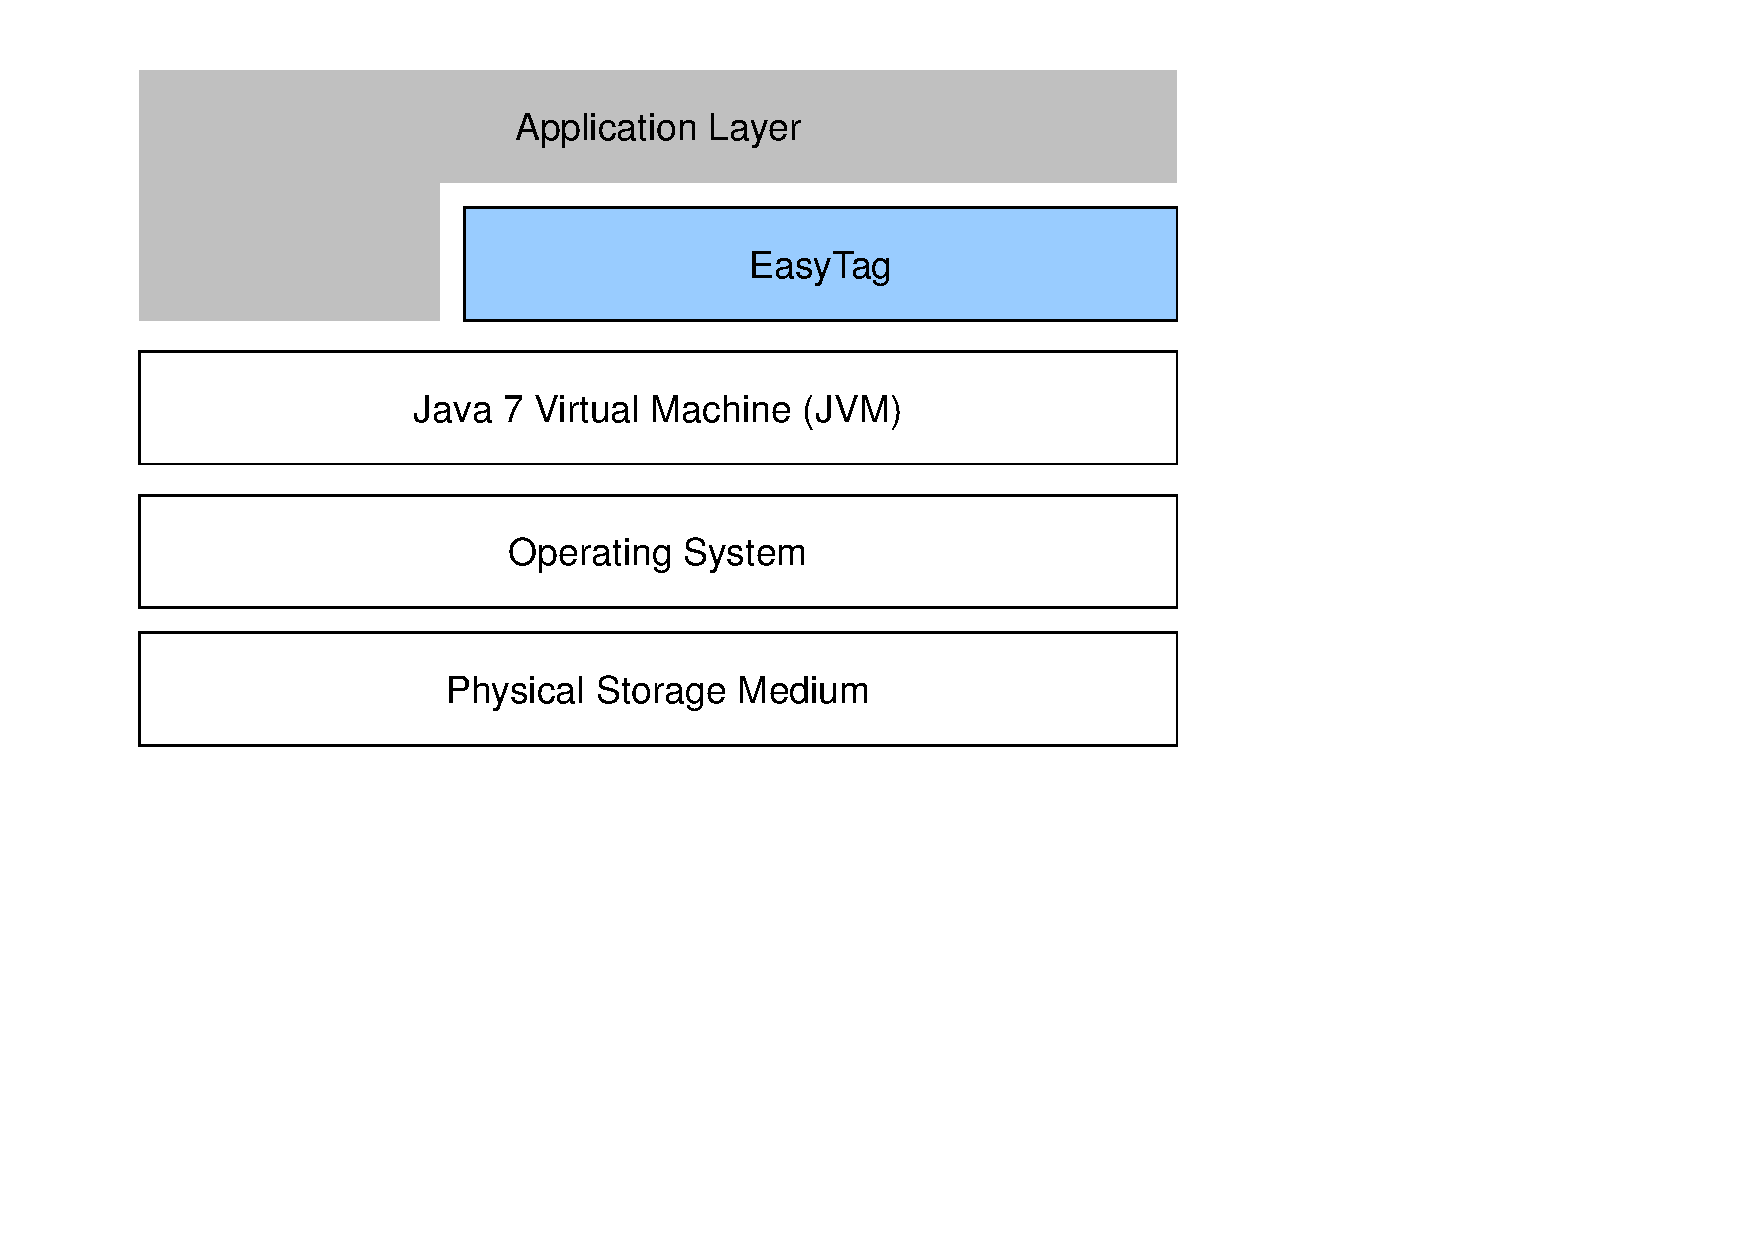
\includegraphics[width=1.00\textwidth]{Figures/Part_II/II_1_TechnicalInfrastructure.pdf}
		\caption{Technical infrastructure of \LibName{}}
	\label{fig:5_3_SCH_TechnicalInfrastructure}
\end{figure}

The technical layers can be interpreted as dependency and communication structure. The application layer is based on \LibName{}, while \LibName{} as well as the application layer uses \JavaVersion{}. Thanks to this, the library and its using applications are platform-independent and can be used on any platform currently supported by Java. \JavaVersion{} accesses the operating system, which offers services to access the physical medium.

However, \LibName{} is only developed for \JavaVersion{} and cannot be used by applications requiring earlier versions.

Each layer only accesses the neighouring layer.

%-----------------------------------------------------------------------------------------------
%		Technische Basiskomponenten
%-----------------------------------------------------------------------------------------------

\section{Technical Base Components}
\label{sec:TechnicalBasis}

Technical base components are just helpers providing a framework and basis for the functional components of \LibName{}. With ``functional'' we are referring to the tasks of the library, i.e. reading and writing metadata and reading container data. The necessary base components are:
\begin{itemize}
	\item Logging
	\item Service-Locator to achieve a component oriented architecture
	\item Utility
	\item Maintaining extensions
\end{itemize}

Details of these components are given in \SectionLink{sec:Design}.

%###############################################################################################
%###############################################################################################
%
%		File end
%
%###############################################################################################
%###############################################################################################